\documentclass[article]{jss}

\author{Bernard Banyuls\\Universidad Complutense de Madrid}
\Plainauthor{Bernard Banyuls}

\title{\pkg{convergence-clubs}: Phillips--Sul Club Convergence Analysis in \proglang{Python}}
\Plaintitle{convergence-clubs: Phillips-Sul Club Convergence Analysis in Python}
\Shorttitle{\pkg{convergence-clubs}}

\Abstract{
  Countries and regions often converge towards different paths rather than a common one,
  and the log $t$ test and clustering algorithm of Phillips and Sul identify these
  convergence clubs. The method is available in \proglang{R} as \pkg{ConvergenceClubs} and
  in \proglang{Stata} as \pkg{psecta}, but not in \proglang{Python}. \pkg{convergence-clubs}
  implements it with \pkg{numpy} and \pkg{pandas}, reproduces the \proglang{R} results to
  within $10^{-8}$, and reproduces the \proglang{Stata} classifications of eight published
  panels. Because the clubs the algorithm finds depend on several settings, the package also
  quantifies that dependence, through sensitivity analysis, bootstrap confidence in each
  membership and clubs estimated over rolling windows. This article describes the method,
  the design of the package and the checks of its correctness, and illustrates its use on
  a panel of GDP for 152 countries.
}

\Keywords{club convergence, log $t$ test, Phillips--Sul, economic growth, \proglang{Python}}
\Plainkeywords{club convergence, log t test, Phillips-Sul, economic growth, Python}

\usepackage{graphicx}
\usepackage{booktabs}
\graphicspath{{figures/}}

\Address{
  Bernard Banyuls\\
  Universidad Complutense de Madrid\\
  Madrid, Spain\\
  E-mail: \email{bbanyuls@ucm.es}\\
  URL: \url{https://github.com/bbanyuls/club-convergence}
}

\begin{document}

\section{Introduction} \label{sec:intro}

Whether poor economies catch up with rich ones is among the oldest questions in growth
empirics. The log $t$ test of \citet{PhillipsSul2007} replaces the assumption of a single
common growth path with a model in which each unit has a transition path to its own
long-run level, and tests whether the cross-sectional dispersion of those paths shrinks.
When the test rejects convergence for the whole panel, a clustering algorithm
\citep{PhillipsSul2009} partitions the units into \emph{convergence clubs}, each of which
passes the test. The procedure is used in applied work on income, productivity, energy and
research spending \citep[for example][]{BanyulsVides2025}.

Two implementations are widely used: the \proglang{R} package \pkg{ConvergenceClubs}
\citep{SicheraPizzuto2019} and the \proglang{Stata} package \pkg{psecta}
\citep{Du2017}. They differ in choices the original papers leave open, so that a
classification depends on which one produced it. A researcher working in \proglang{Python}
has had to leave the language or reimplement the method.

This article presents \pkg{convergence-clubs}, a \proglang{Python} package with three aims.
First, to implement the method so that its results match both existing implementations,
with the differences between them explicit and selectable. Second, to treat the number
and membership of clubs as an estimate with uncertainty, since they change with the
settings. Third, to place the clubs in context with the classical convergence measures.
Section~\ref{sec:method} summarises the method, Section~\ref{sec:design} describes the
package, Section~\ref{sec:validation} reports the validation, and
Section~\ref{sec:illustration} illustrates a complete analysis.

\section{The method} \label{sec:method}

Let $X_{it}$ be the (usually log and trend-filtered) observation of unit $i$ at time $t$,
for $i = 1, \dots, N$ and $t = 1, \dots, T$. The relative transition path is
$h_{it} = X_{it} / (N^{-1} \sum_i X_{it})$ and the cross-sectional variation is
$H_t = N^{-1} \sum_i (h_{it} - 1)^2$. Under convergence $H_t$ falls over time, and the
log $t$ regression
\begin{equation}
  \log \frac{H_1}{H_t} - 2 \log \log t = a + b \log t + u_t, \qquad t = \lfloor rT \rfloor, \dots, T,
\end{equation}
gives the test of the null $b \ge 0$ against divergence, rejected when the $t$-statistic
of $\hat{b}$ is below $-1.65$. The regression uses a heteroskedasticity and autocorrelation
consistent (HAC) covariance, with the fixed-bandwidth (FQSB) or the \citet{Andrews1991}
data-driven (AQSB) quadratic spectral estimator. The trimming $r$ discards the first
periods.

The clustering sorts units by their final observations, forms a core group of top-ranked
units chosen by the log $t$ statistic, adds units one at a time while the club keeps
passing the test (with $c^*$ as a sign threshold), and repeats on the remaining units.
Clubs that converge together are then merged, with the rules of
\citet{PhillipsSul2009} (PS) or \citet{vonLynckerThoennissen2017} (vLT).

\section{The package} \label{sec:design}

The package needs only \pkg{numpy} and \pkg{pandas}; plots, interactive charts and maps
are optional extras installed with \code{pip install "convergence-clubs[plot]"}. Its
functions follow those of the \proglang{R} package, so \proglang{R} code translates
directly.

\begin{CodeChunk}
\begin{CodeInput}
>>> import numpy as np
>>> import convergence_clubs as cc
>>> gdp = cc.load_gdp()
>>> data = cc.hp_filter(np.log(gdp), lamb=400)
>>> clubs = cc.find_clubs(data)
>>> clubs.summary()
\end{CodeInput}
\begin{CodeOutput}
        n_units   beta  std_err  t_value  p_value  converges  cstar
club
club1        50  0.382    0.041    9.282    1.000       True    0.0
club2        30  0.240    0.035    6.904    1.000       True    0.0
club3        21  0.110    0.032    3.402    1.000       True    0.0
club4        24  0.131    0.064    2.055    0.980       True    0.0
club5        14  0.190    0.111    1.701    0.956       True    0.0
club6        11  1.003    0.166    6.024    1.000       True    0.0
club7         2 -0.470    0.842   -0.559    0.288       True    0.0
\end{CodeOutput}
\end{CodeChunk}

Results are immutable objects that record the settings used. The argument
\code{convention="Stata"} switches every choice at once to the \pkg{psecta} behaviour
(the core group by largest $t$, $c^*$ raised automatically, and a 0.3 trimming);
individual choices are also arguments. \code{sensitivity()} re-estimates the clubs over a
grid of settings, \code{bootstrap()} perturbs the data, \code{rolling\_clubs()} follows the
clubs through time, and the classical measures ($\beta$- and $\sigma$-convergence,
distribution dynamics, a pairwise test, an ordered logit of club membership) are
provided alongside. Long analyses run in parallel with \code{n\_jobs} and return the same
result for any number of workers.

\section{Validation} \label{sec:validation}

\textbf{Against \proglang{R}.} Test statistics, club sizes and memberships are compared
with fixtures generated by \pkg{ConvergenceClubs} 2.2.5, on simulated panels and on the
GDP panel, to within $10^{-8}$. The comparison is repeated weekly against the current
release of the \proglang{R} package. The GDP example reproduces the published table of
\citet{SicheraPizzuto2019}: seven clubs of 50, 30, 21, 24, 14, 11 and 2 countries,
and six after merging.

\textbf{Against \proglang{Stata}.} With \code{convention="Stata"}, the package reproduces
the \pkg{psecta} and \pkg{imergeclub} classifications of all eight panels in
\citet{Mendez2020} (two samples and four variables), both before and after merging.
Under the \proglang{R} conventions two of the eight differ, and each is explained by one
of the two \proglang{Stata} rules.

\textbf{Known differences.} Two inconsistencies were found in \pkg{ConvergenceClubs}
2.2.5: a stale model at the cap of $c^*$, and a second merging test that ignores the HAC
method. Both were reported upstream with a fix. For the second, the package follows the fix.
The documentation lists these differences.

All numbers in this article are reproduced by the script \code{paper/jss/replication.py}
in the repository, which stops if any of the comparisons above fails. The test suite
has 446 tests with full line coverage and runs on the oldest and newest supported
dependency versions.

\section{Illustration} \label{sec:illustration}

\subsection{The clubs}

On the GDP panel (152 countries, 1970--2003, log and HP-filtered with $\lambda = 400$)
the whole sample diverges: the log $t$ statistic is $-159.6$. The algorithm finds seven
clubs of 50, 30, 21, 24, 14, 11 and 2 countries, each passing the test, and the PS rule
merges the fourth and fifth, leaving six. Figure~\ref{fig:paths} shows the relative
transition paths of the six merged clubs. The clubs separate in the way the method
predicts: the paths of the richest clubs drift up and stay flat, and those of the poorest
decline.

\begin{figure}[t!]
  \centering
  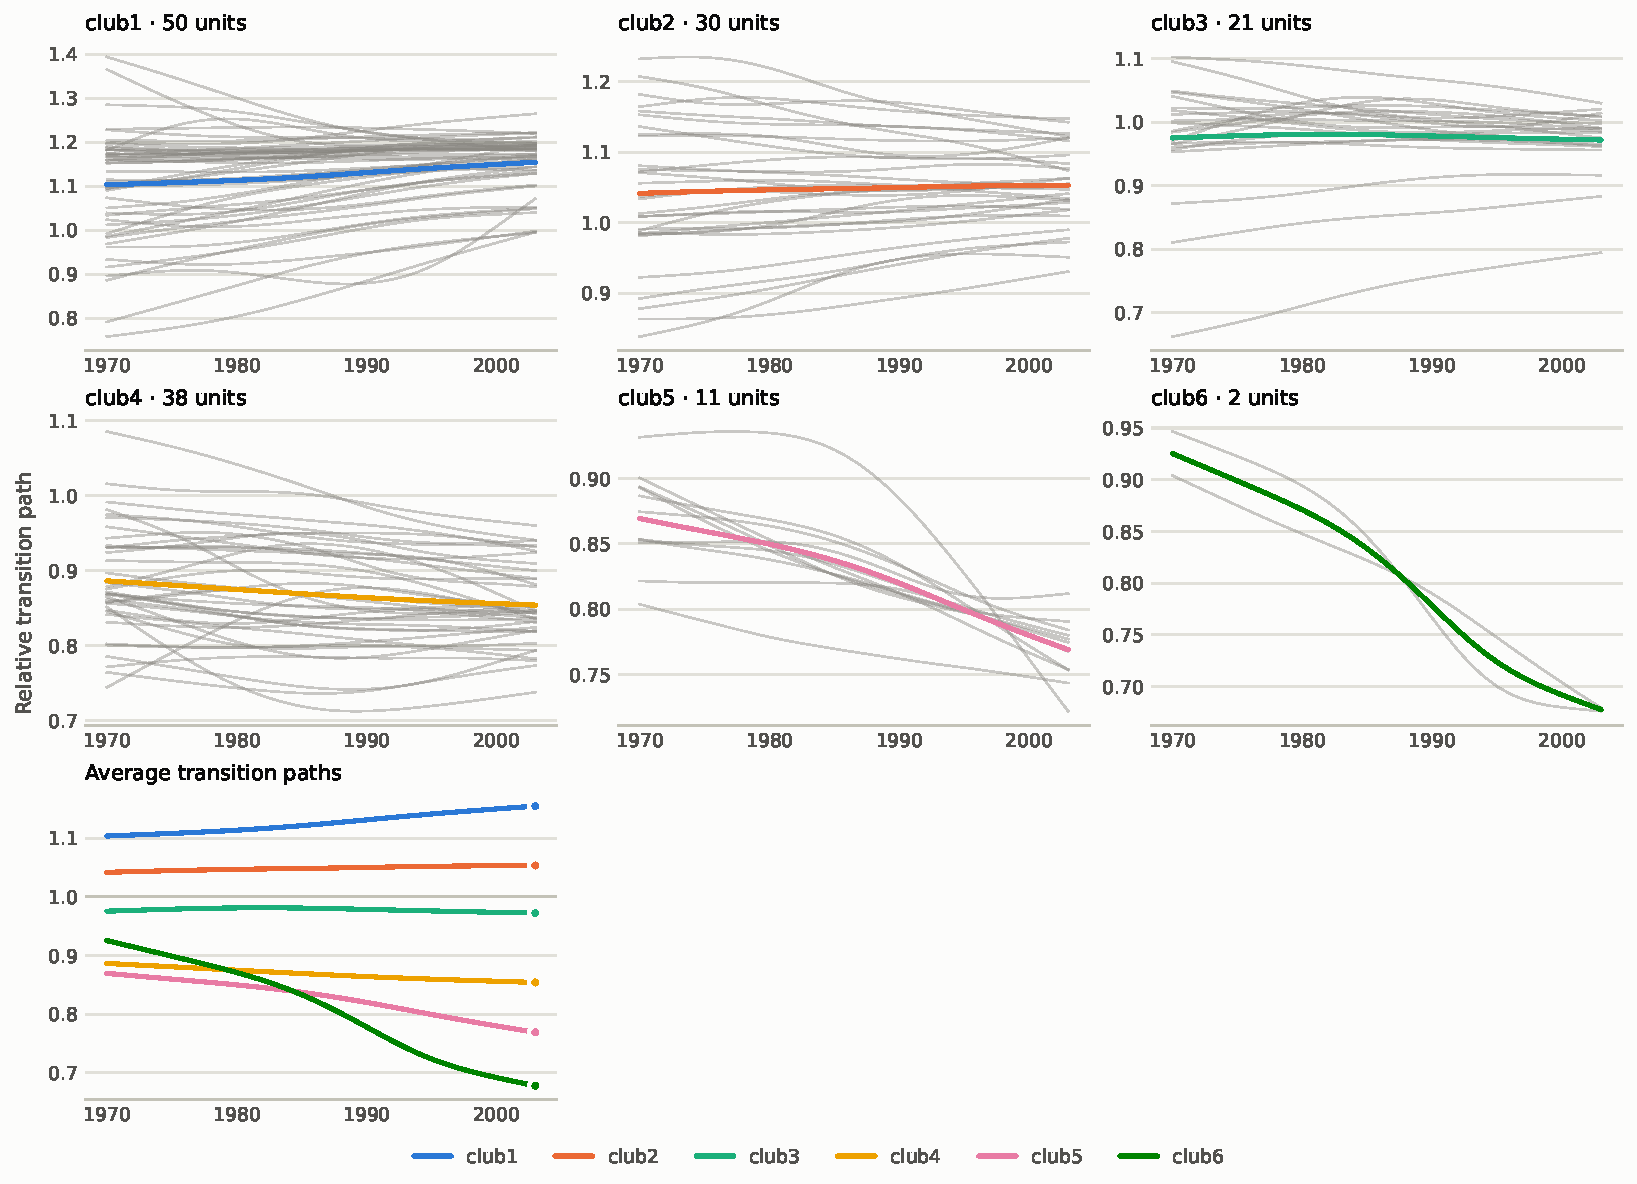
\includegraphics[width=\textwidth]{transition_paths.pdf}
  \caption{Relative transition paths $h_{it}$ of the six clubs after PS merging, with the
    club average in colour and the last panel comparing the averages.}
  \label{fig:paths}
\end{figure}

\subsection{How firm are they?}

The number of clubs is not a fixed fact of the data. Over sixteen combinations of
trimming (four values), HAC method (two) and merging (none or PS), the package finds
between four and nine clubs. For each country, the share of runs in which it stays with
its baseline club mates has a median of 0.84 and a minimum of 0.41
(\code{cc.sensitivity(...).stability()}).

The bootstrap gives a second view. In 200 resamples of 80\% of the units
(\code{cc.bootstrap(data, 200, merge="PS", seed=0)}), 52 of the 152 countries stay with
their club mates in fewer than 80\% of the runs. Figure~\ref{fig:stability} shows
the share for each country by club.

\begin{figure}[t!]
  \centering
  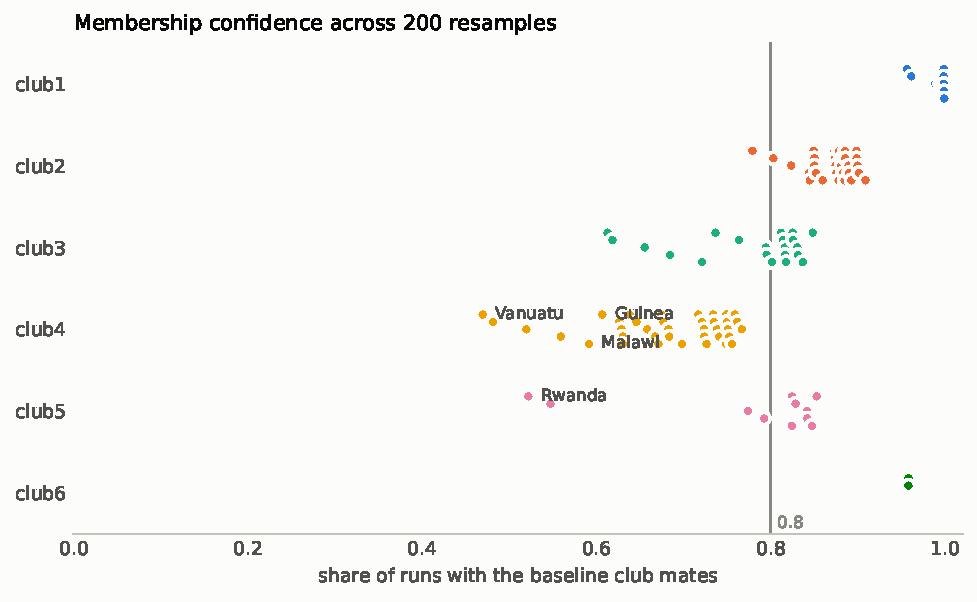
\includegraphics[width=0.8\textwidth]{bootstrap_stability.pdf}
  \caption{Share of 200 bootstrap resamples in which each country stays with its
    baseline club mates, by club. The line marks 0.8.}
  \label{fig:stability}
\end{figure}

Reporting this is the point of these tools. Two analyses with the same data and
different but defensible settings can report different numbers of clubs, and the
published classifications rarely say how much of the result survives. The same method
was used for research spending in the European Union \citep{BanyulsVides2025}.

\section{Summary} \label{sec:summary}

\pkg{convergence-clubs} makes the Phillips--Sul method available in \proglang{Python},
matches the two existing implementations on published results, and adds the tools
to judge how robust the clubs are. The package is on PyPI and the source and
documentation are at \url{https://github.com/bbanyuls/club-convergence}.

\section*{Computational details}

The results were obtained with \proglang{Python} 3.13, \pkg{numpy}, \pkg{pandas} and
\pkg{convergence-clubs} 0.1.2, and the reference results with \proglang{R} 4.6.1 and
\pkg{ConvergenceClubs} 2.2.5. The package is licensed under GPL-3.0-or-later.

\section*{Acknowledgments}

Generative AI (Claude Code, Anthropic) was used in the development of the software and in
drafting this article. The author decided the design and the validation strategy,
reviewed all output and is responsible for the work.

\bibliography{convergence-clubs}

\end{document}
